\documentclass[tikz]{standalone}

\usepackage{tikz}
\usetikzlibrary{shapes.arrows}

\usepackage{graphicx}

\begin{document}
    \begin{tikzpicture}
        \node[visible on=<3-6>] (sampled_pc) {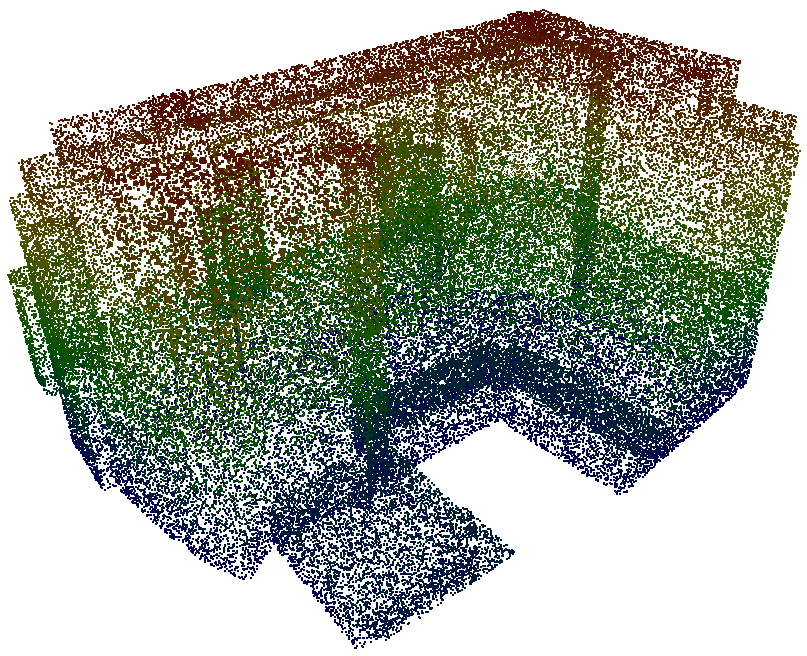
\includegraphics[width=2cm]{images/context/sampled_pc}};
        \path (sampled_pc.east) node[anchor=west, visible on=<3-6>] (3d_reconstruction) [
            draw,
            single arrow,
            color=blue,
            minimum height=1cm
        ] {3D urban modeling};

        \path (3d_reconstruction) node[visible on=<1>] (aerial_images) {\includegraphics[width=4cm]{example-image}};
        \path (aerial_images) node[visible on=<2>] (lidar_pcs) {\includegraphics[width=4cm]{example-image}};

        \path (3d_reconstruction) node[visible on=<4>] (human_op) {
\includegraphics[width=2cm]{images/context/operator}};
        \path (human_op) node[visible on=<5>] (automatic) {
\includegraphics[width=2cm]{images/context/automatic}};

        \path (3d_reconstruction.east) node[anchor=west, visible on=<3-6>] (3d_model) {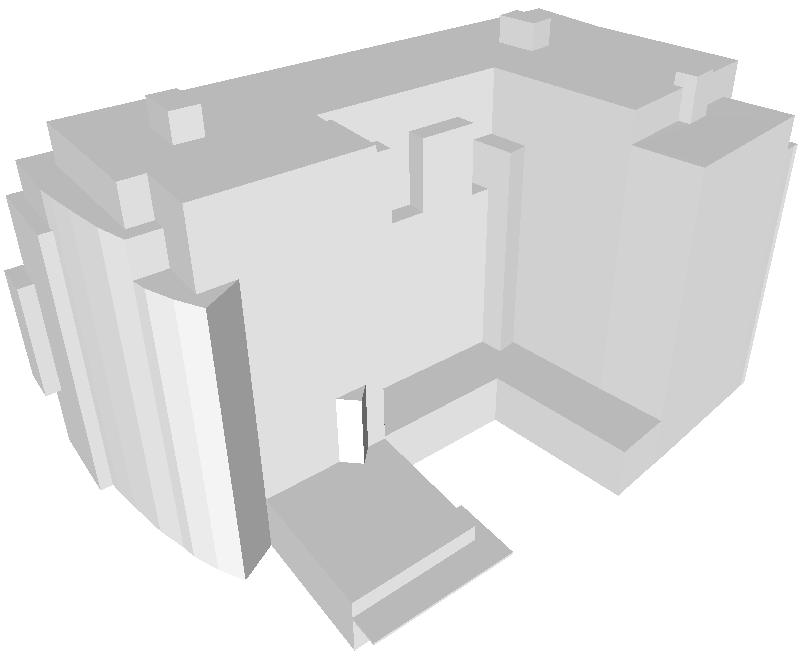
\includegraphics[width=2cm]{images/context/3d_model}};

        \path (3d_reconstruction) node[visible on=<7->] (3d_model_quality) {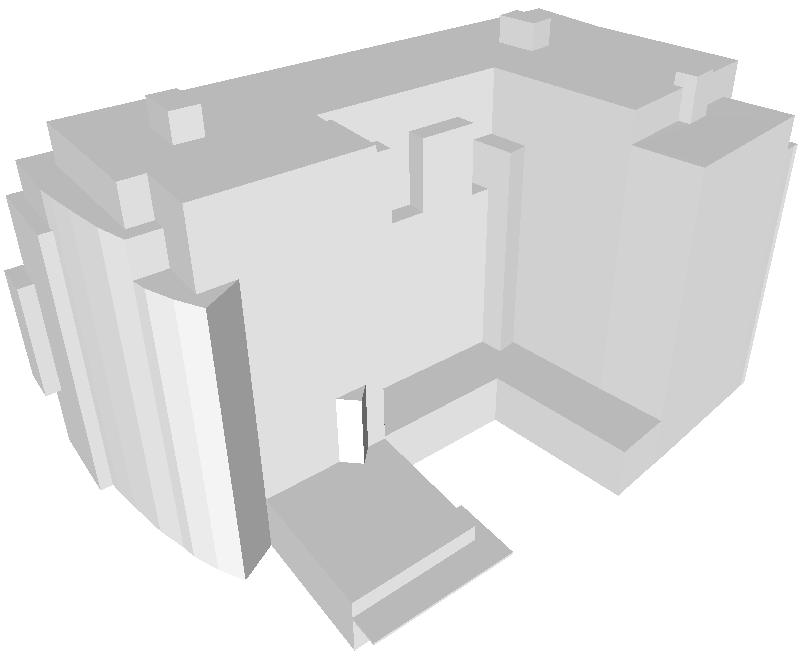
\includegraphics[width=2cm]{images/context/3d_model}};

        \path (3d_model_quality.south) node[anchor=north, red, visible on=<8->] (evaluation) {How good is this model?};
    \end{tikzpicture}
\end{document}